\documentclass[twocolumn]{iopjournal}

\usepackage{amsmath,amssymb,amsfonts}

\fancyhfoffset[L]{0mm}
\setlength{\marginparwidth}{0pt}
\setlength{\marginparsep}{0pt}

% ==========================================
% ZENODO PREPRINT HEADERS (ACTIVE)
% ==========================================
\renewcommand{\articletype}[1]{%
  {\vspace*{-8mm}\noindent \Large \sf Preprint}\par
  \vspace*{6mm}\noindent{\scriptsize \sf{\bfseries \MakeUppercase{#1}}}}

\fancyhead[L]{}
\fancyhead[R]{}

\begin{document}

\articletype{Letter}

\title{Gravity Field Dynamics: Field Closure of the Tetrad Frame}

\author{Stephen Nelson}

\affil{Field Dynamics Research}

\ead{stephen@fielddynamics.org}

\begin{abstract}
This letter proves that the torsion-free condition
$\Gamma^\lambda_{\mu\nu} = \Gamma^\lambda_{\nu\mu}$ retains
the $s = +1$ projection of the coupling polynomial
$f(K,s) = 1 + sK + K^2$ and discards the $s = -1$
projection: the retained count per face is
$(f(K,{+}1){-}1)/2 = 10$, the discarded count is
$(f(K,{-}1){-}1)/2 = 6$, giving 40~retained and
24~discarded across four faces.  The polynomial and the
constitutive law $\mu(x) = x/(x{+}1)$ were derived in the
companion letters from the tetrad
equation~\cite{Nelson2026a,Nelson2026b}; the companion
identification of $s = +1$ with TetA and $s = -1$ with
TetB~\cite{Nelson2026b} means the 24~discarded components
are the second root of the tetrad equation.  Restoring them
yields the full $K^3 = 64$ component connection.  The
constitutive law partitions the restored components spatially:
the two partition surfaces cross at the MOND transition
scale, and the closed partition $\mu + (1{-}\mu) = 1$
produces an emergent disk-and-bulge morphology that requires
both roots.  Integration of $\mu$ via the standard
AQUAL identity yields the unique scalar-sector energy
functional
$F(y) = y - 2\sqrt{y} + 2\ln(1{+}\sqrt{y})$.  Polynomial
long division of the integrand shows that the three terms
of $F$ reproduce the three structural levels of the coupling
polynomial, confirming its rank structure from a variational
direction.  The constitutive law determines the
Gravity Field Dynamics covariant action; the action determines
the dynamics; no step in this chain involves a free parameter.
\end{abstract}

% ==================================================================

\section{The torsion-free projection}

\begin{figure}[!t]
\centering
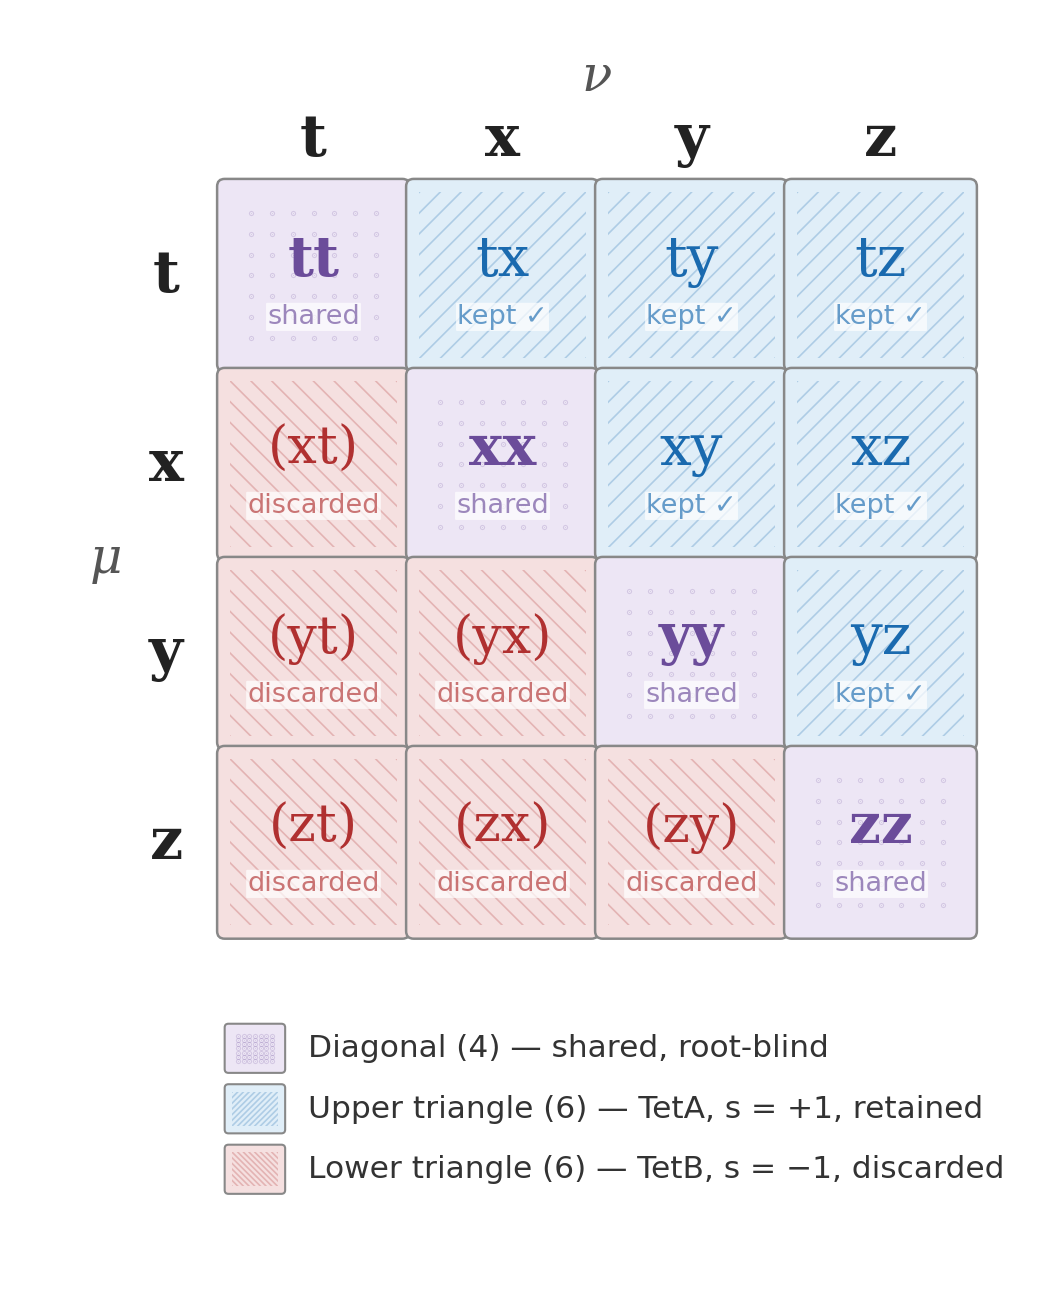
\includegraphics[width=\columnwidth]{fig1_matrix.png}
\caption{The $(\mu,\nu)$ matrix for one observation face
$\lambda$.  Diagonal entries (bold) are shared: the metric
cannot distinguish the two roots there.  Upper-triangle
entries belong to the $s = +1$ projection (TetA, retained).
Lower-triangle entries belong to the $s = -1$ projection
(TetB, discarded by the torsion-free condition).  The same
pattern repeats for all four values of $\lambda$.}
\label{tab:matrix}
\end{figure}

The affine connection on a $K$-dimensional frame has three
indices $\Gamma^\lambda_{\mu\nu}$, each running from 0 to
$K - 1$.  The total number of components is $K^3$.  At
$K = 4$, this gives 64~\cite{Nelson2026b,Hehl1976}.

The torsion-free condition forces symmetry of the lower pair:
\begin{equation}
  \Gamma^\lambda_{\mu\nu} = \Gamma^\lambda_{\nu\mu}.
  \label{eq:torsion_free}
\end{equation}
The companion letters established the structural
prerequisites.  Letter~1~\cite{Nelson2026a} proved that
the tetrad equation produces a stellated octahedron geometry
with structural constants $K = 4$, $D = 3$, selected by the
uniqueness equation $2(D{+}1) = 2^D$.

Letter~2~\cite{Nelson2026b} showed that
the tetrad equation
$g_{\mu\nu} = \eta_{ab}\,e^a{}_\mu\,e^b{}_\nu$ contains
three structural ingredients at ranks 0, 1, and~2 on the
frame space, with graded dimensions $K^0 = 1$ (the scalar
closure, or field origin, from which the rank structure
begins), $K^1 = K$, and $K^2$.  The tetrad equation is quadratic in the frame
field and admits two roots related by spatial parity
$e^i{}_\mu \to -e^i{}_\mu$ ($i = 1,2,3$).  The scheme (solution space) of
this quadratic equation has exactly two connected components
in the spatial sector; there is no consistent way to retain
one and discard the other, because both satisfy the same
defining equation with the same
metric~\cite{Nelson2026a}.  The standard convention of
selecting one signature orientation is a projection onto one
component, not an elimination of the other.  Because the
metric is bilinear in the frame field, both roots produce the
same $g_{\mu\nu}$; the metric alone cannot distinguish
them.  Under parity,
a rank-$r$ tensor transforms with sign $(-1)^r$.  Ranks~0
and~2 are parity-even; rank~1 is parity-odd.  The rank-1
vielbein is therefore the only ingredient whose sign changes
when the two roots are exchanged, sending $s \to -s$ and
identifying TetA with $s = +1$ and TetB with $s = -1$.  The
coupling polynomial is
\begin{equation}
  f(K,s) = 1 + sK + K^2.
  \label{eq:poly}
\end{equation}
Because that scheme contains both roots by
construction~\cite{Nelson2026a}, the second root cannot be
removed from the equation; the torsion sector is
the necessary carrier of the two-root distinction, because
the metric $g_{\mu\nu} = \eta_{ab}\,e^a{}_\mu\,e^b{}_\nu$
is bilinear in the frame field and therefore invariant under
$e^i \to -e^i$: a torsion-free connection, being uniquely
determined by this invariant metric, inherits that invariance
and cannot resolve which root the frame
occupies~\cite{Nelson2026b}.  Exchange symmetry between the two
roots determines the field fraction carried by TetB as
$1 - \mu(x) = 1/(x{+}1)$ at every
radius~\cite{Nelson2026b}.  Together, these results mean
that the components projected out by the torsion-free
condition are not free slots: their existence is algebraically
necessary, their carrier is uniquely the torsion sector, and
their value is algebraically determined.

For each value of the upper index $\lambda$, the lower pair
$(\mu, \nu)$ forms a $K \times K$ matrix with $K^2 = 16$
entries.  Of these, $K = 4$ are diagonal ($\mu = \nu$) and
$K^2 - K = 12$ are off-diagonal.  The off-diagonal entries
form $\tfrac{1}{2}(K^2 - K) = 6$ mirror pairs, each
consisting of $(\mu, \nu)$ and $(\nu, \mu)$.  The
torsion-free condition~(\ref{eq:torsion_free}) forces the two
members of each pair to be equal, retaining the symmetric
combination and discarding the antisymmetric combination.  The
count per face is therefore:
\begin{align}
  \text{Retained:} \quad
    & K + \frac{K^2 - K}{2} = \frac{K^2 + K}{2} = 10,
    \label{eq:kept} \\[4pt]
  \text{Discarded:} \quad
    & \frac{K^2 - K}{2} = 6.
    \label{eq:disc}
\end{align}
Across $K = 4$ observation faces: $4 \times 10 = 40$ retained,
$4 \times 6 = 24$ discarded, $4 \times 16 = 64$ total.
The same split can be read from the polynomial side.
The coupling polynomial~(\ref{eq:poly})
evaluates to $f(K,{+}1) = 21$ at the TetA state and
$f(K,{-}1) = 13$ at the TetB state.  The field-origin term
$K^0 = 1$ corresponds to the diagonal entries ($\mu = \nu$),
which have no mirror partner and are invariant under index
exchange; they belong to neither projection but are shared
(root-blind).  Subtracting this term and halving the remainder
for mirror-pair degeneracy:
\begin{align}
  \text{Retained (TetA):} \quad
    \frac{f(K,{+}1) - 1}{2}
    &= \frac{K^2 + K}{2} = 10,
    \label{eq:poly_kept} \\[6pt]
  \text{Discarded (TetB):} \quad
    \frac{f(K,{-}1) - 1}{2}
    &= \frac{K^2 - K}{2} = 6.
    \label{eq:poly_disc}
\end{align}
The combinatorial formula for the symmetric/antisymmetric
split of a $K \times K$ matrix is the coupling polynomial
evaluated at its two opposite states, with the field-origin
term removed and the mirror-pair degeneracy halved.  The
$\pm K$ that separates 10 from 6 is the $sK$ term of the
polynomial: the parity-odd rank-1 contribution.

The torsion-free condition therefore retains the $s = +1$
projection of the coupling polynomial and discards the
$s = -1$ projection.  Since the companion
letters~\cite{Nelson2026a,Nelson2026b} proved
that spatial parity sends $s \to -s$, identifying TetA with
$s = +1$ and TetB with $s = -1$, the retained projection is
the TetA contribution and the discarded projection is TetB.
The 24~components removed by the torsion-free condition are
the second root of the tetrad equation, carrying a distinct
field fraction $1 - \mu(x)$ at every
radius~\cite{Nelson2026b}.  Restoring them
returns the full $K^2 = 16$ components per face and the full
$K^3 = 64$ component connection.

The full 64-component connection achieves
\textit{field closure}: both roots of the tetrad equation
contribute, the partition $\mu + (1{-}\mu) = 1$ holds at
every radius, and the field response is self-consistent
without external mass.  This is distinct from Einstein's
notion of a ``complete field theory'' (in which the equations
of motion follow from the field equations without independent
postulates) and from geodesic completeness (the extendibility
of geodesics to infinite affine parameter).  Field closure
refers specifically to the connection: whether all $K^3$
components of the affine connection are active, or whether a
subset has been set to zero by constraint.
Einstein--Cartan theory~\cite{Hehl1976} restores torsion but
couples it algebraically to spin, so that it vanishes in
vacuum.  The present framework restores torsion with an
acceleration-dependent partition: the 24~antisymmetric
components carry the fraction $1 - \mu(x)$ of the field
response, which is nonzero wherever $x$ is finite.
The source of torsion in this framework is not intrinsic spin
but the constitutive partition between the two roots of the
tetrad equation: a kinematic, acceleration-dependent
allocation that persists in vacuum.

% ==================================================================

\section{The partition in space}

The companion letter~\cite{Nelson2026b} derived the partition
between the two projections from exchange symmetry:
\begin{align}
  \text{TetA ($s = +1$):} \quad & \mu(x) = \frac{x}{x + 1},
  \label{eq:mu} \\[4pt]
  \text{TetB ($s = -1$):} \quad & 1 - \mu(x) = \frac{1}{x + 1},
  \label{eq:tetb}
\end{align}
where $x = g/a_0$ is the dimensionless acceleration.  The
torsion-free condition conflates the two projections, treating
both members of each mirror pair as carrying the same value.
Eqs~(\ref{eq:mu})--(\ref{eq:tetb}) show they carry equal
fractions only at $x = 1$ ($\mu = 1/2$).  At every other
radius, the conflation discards a nonzero TetB contribution:
at the galactic centre ($x \gg 1$), the discarded fraction is
small; at the rim ($x \ll 1$), it is the majority of the
field response.

What does the restored $s = -1$ projection look like
spatially?  The answer is Figure~\ref{fig1}.

\begin{figure}[t]
\centering
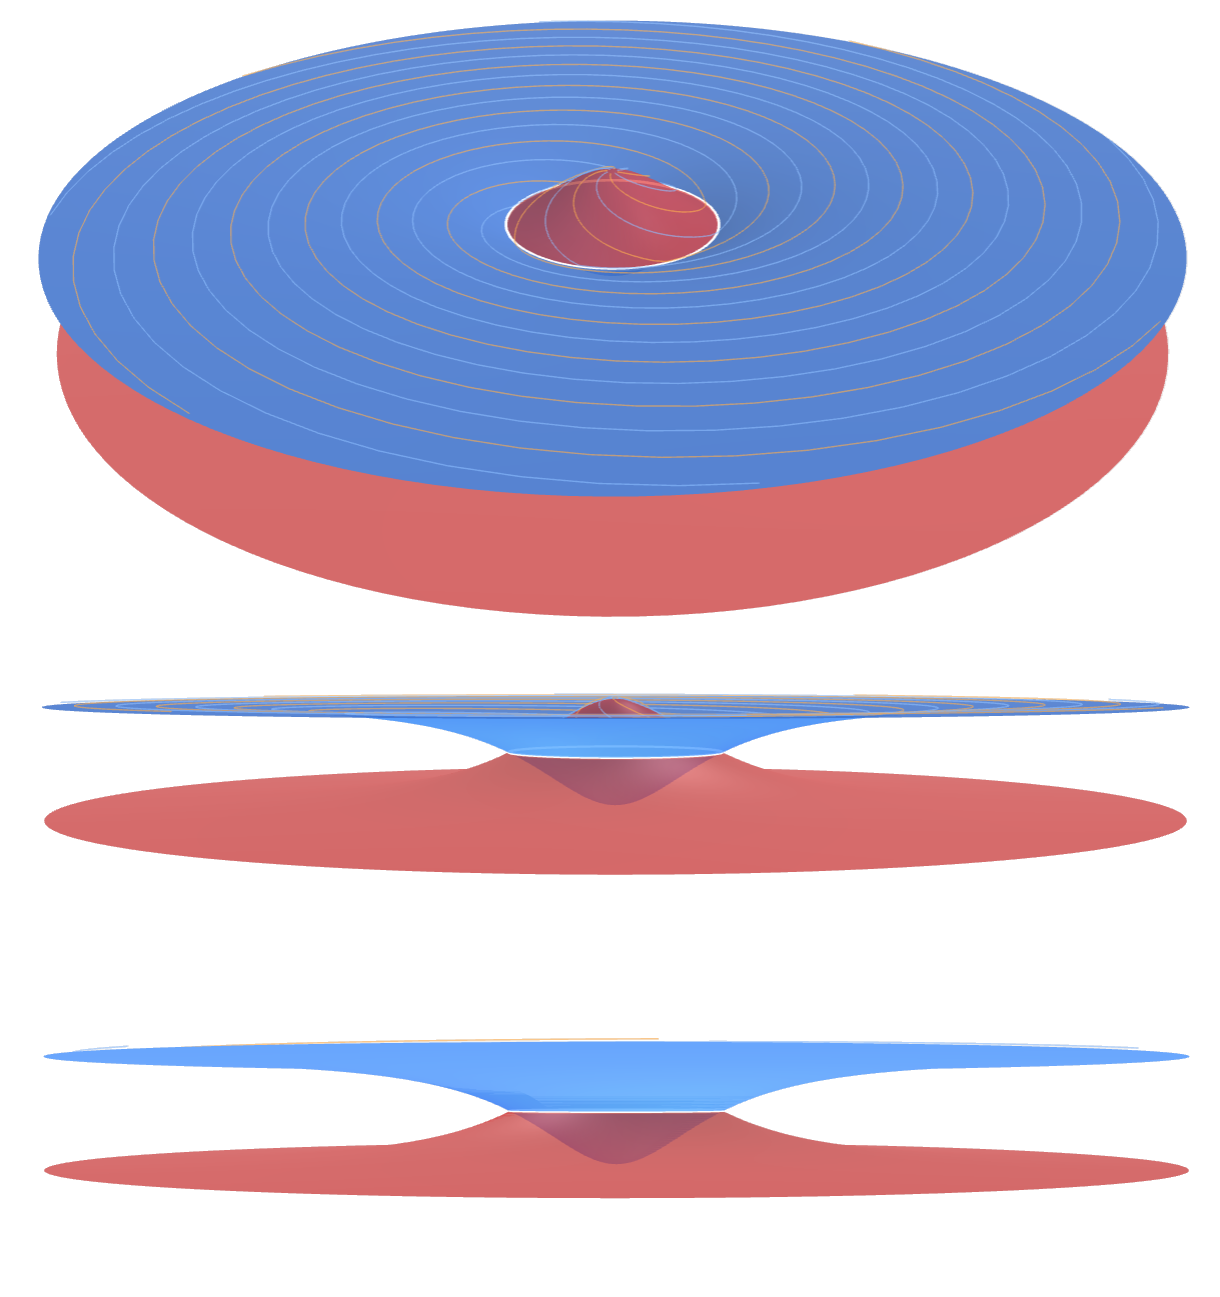
\includegraphics[width=\columnwidth]{fig2_tetrad_partition}
\caption{The constitutive law $\mu(x) = x/(x{+}1)$,
partitioned between the two projections identified by the
coupling polynomial.  Blue: the $s = +1$ projection $\mu$
(TetA, retained by general relativity).  Red: the $s = -1$
projection $1 - \mu$ (TetB, removed by the torsion-free
condition).  At every radius, blue~$+$~red~$= 1$.  The two
surfaces are exact mirrors, crossing at $x = 1$ where both
projections contribute equally ($\mu = 1/2$); the white ring
marks this locus.  The polynomial identifies which projection
is which; the constitutive law determines how much each
carries at every radius.}
\label{fig1}
\end{figure}

Figure~\ref{fig1} renders each projection as its own surface
of revolution.  The radial domain extends outward from the
central axis, with the dimensionless acceleration
$x = g/a_0$ decreasing toward the rim.  At each radius, the
value of the blue surface is $\mu(x)$ and the value of the
red surface is $1 - \mu(x)$.  The surfaces are azimuthally
symmetric because the constitutive law depends only on the
scalar acceleration, not on angle.  Because
$\mu + (1{-}\mu) = 1$, the two surfaces are exact mirrors:
they cross at $x = 1$ where both equal $1/2$, and the white
ring marks this locus.  Figure~\ref{fig1} is therefore not a
heuristic sketch but the constitutive law itself rendered
over radius.
A theory restricted to the 40~Christoffel components sees
only the blue surface; the red surface is the field response
it discards.

Every gravitationally bound system has an acceleration
profile that is strongest at the centre and weakens
outward; for any concentrated mass distribution this follows
from Gauss's law.  The constitutive law
$\mu(x) = x/(x{+}1)$ is a monotonic function: higher
acceleration always maps to a larger TetA fraction, and lower
acceleration always maps to a larger TetB fraction.  Where
$x$ is large (the centre), $\mu$ is near unity and the blue
surface carries nearly the full field response.  Where $x$ is
small (the rim), $1 - \mu$ is near unity and the red surface
carries it.  The two surfaces cross at $x = 1$, creating a
morphological boundary between a concentrated interior and
an extended exterior.  Neither surface alone produces this
structure: TetA alone is a monotonic decay; TetB alone is a
flat plateau.  The disk-and-bulge configuration visible in
Figure~\ref{fig1} is emergent from the closed partition
$\mu + (1{-}\mu) = 1$ and requires both roots.  The
morphology is not fitted; it is the constitutive law's
prediction for the field configuration of any bound mass
distribution.  The crossover radius is set by $x = 1$,
independent of galaxy mass or morphology.  Because the
constitutive law applies to any gravitationally bound system,
Figure~\ref{fig1} should be read as a spatial rendering of
that law, not as a new fit.

The value of each surface in Figure~\ref{fig1} is the
fraction of the gravitational field response carried by that
root at each radius.  The two fractions sum to unity
everywhere: the total field response is not enhanced but
redistributed between the two roots.  The two surfaces are
not independent distributions.  The interior (where $\mu$
dominates) and the exterior (where $1 - \mu$ dominates) are
coupled through the partition constraint
$\mu + (1{-}\mu) = 1$: the interior drives the field
configuration and the exterior continues that drive; the two
together produce the net field.  The outer
share is not an added component; it is the outward
continuation of the same closed field.  The field strength
observed at any exterior radius includes a contribution
driven by the interior that exterior matter alone does not
account for.  The shape of this coupled
configuration depends on the enclosed mass profile through
$x(r) = g(r)/a_0$: a more concentrated mass produces a
sharper interior spike and correspondingly broader exterior
response; a more extended distribution produces a gentler
interior and a shallower exterior.  The textbook
decomposition of the full connection into Christoffel plus
contorsion corresponds, at the level of field magnitudes, to
the partition into $\mu$ and
$1 - \mu$~\cite{Nelson2026b}.  Figure~\ref{fig1} is that
decomposition rendered spatially.

The white ring sits at $x = 1$, where $\mu = 1/2$.  This is
the locus where both projections contribute equally to the
field response.  Inside the ring, the Christoffel sector
dominates: general relativity is accurate and Keplerian
decline holds.  Outside the ring, the torsion sector
dominates: the field response that general relativity
discards becomes the majority.  This crossover is the MOND
transition scale $a_0$~\cite{Milgrom1983}.  It is not a
fitted parameter.  It is the geometric midpoint of the
exchange-symmetric partition, the point where the odds ratio
$\Omega = \mu/(1-\mu)$ equals unity.

The rate at which the partition shifts between the two
projections is characterised by a logistic identity that
$\mu$ satisfies~\cite{Nelson2026b}:
\begin{equation}
  x\,\frac{d\mu}{dx} = \mu(1 - \mu).
  \label{eq:logistic}
\end{equation}
Under the substitution $t = \ln x$, this becomes
$d\mu/dt = \mu(1-\mu)$: the canonical two-sector transition
law.  The product $\mu(1-\mu)$ on the right-hand side measures
the simultaneous presence of both tetrahedral chambers at a
given radius.  It is the continuous analogue of the octahedral
interaction core, the $s = 0$ state of the coupling
polynomial~\cite{Nelson2026b}.  The transition peaks at the
MOND ring because that is where the core is fully realised:
$\mu(1 - \mu) = 1/4$.

The kinematic consequence follows directly from the partition.
At dimensionless acceleration $x = g_{\mathrm{obs}}/a_0$, the
baryonic acceleration, carried by the Christoffel sector, is
$g_{\mathrm{bar}} = \mu\,g_{\mathrm{obs}}$, giving
\begin{equation}
  g_{\mathrm{bar}} =
  \frac{g_{\mathrm{obs}}^2}{g_{\mathrm{obs}} + a_0}.
  \label{eq:rar}
\end{equation}
At high acceleration ($x \gg 1$):
$g_{\mathrm{bar}} \approx g_{\mathrm{obs}}$, Keplerian
decline, general relativity is accurate.  At low acceleration
($x \ll 1$):
$g_{\mathrm{bar}} \approx g_{\mathrm{obs}}^2/a_0$, flat
rotation curves.  The radial acceleration relation established
empirically by McGaugh, Lelli \&
Schombert~\cite{McGaugh2016}, with 0.057~dex scatter across
175~individual galaxies~\cite{Li2018} and no credible
variation in $a_0$, is reproduced by Eq.~(\ref{eq:rar}) with
no free parameters.

The apparent separation of baryonic and dark components in
Figure~\ref{fig1} is a diagnostic decomposition of one field,
not a claim of two independent physical substances.  It is the
projection of a single 64-component field onto a 40-component
subspace.  The observed gravitational discrepancy at galactic
scales is not in dispute: both the cold dark matter framework
and the present partition reproduce the radial acceleration
relation and the function $\mu(x) = x/(x{+}1)$.  They differ
on what the discrepancy represents.  The cold dark matter
framework interprets it as an invisible mass component,
modelled with approximately spherical
halos~\cite{NFW1996}.  The companion letter proved that the
cold-dark-matter residual and the torsion-sector field
fraction are algebraically identical under the
exchange-symmetric partition: both reduce to
$1/(x{+}1)$~\cite{Nelson2026b}.  The red surface in
Figure~\ref{fig1} is the spatial rendering of that same field
response; its approximately spherical envelope at large
radius is the structure that halo modelling approximates.
The closed tetrad frame identifies it
as the field response of the second tetrahedral chamber,
carried by the 24~torsion components.  This response is not
mass.  It is the topology of the connection: the field
contribution of the second tetrahedral chamber.

% ==================================================================

\section{From partition to action}

The partition developed in Sections~1--2 produces three
physical consequences that distinguish it from the cold
dark matter framework.

\textit{Disk-and-bulge morphology.}  The closed partition, with
both roots active, produces an emergent concentrated interior
and extended exterior whose morphological boundary lies at the
MOND ring $x = 1$.  Neither root in isolation yields this
structure; it requires the crossing of the two partition
surfaces.

\textit{Bounded central density.}  The TetB field fraction
$1/(x{+}1)$ is bounded above by unity for all $x$.  The
torsion-sector field acceleration never exceeds $a_0$.  The NFW
profile diverges as $r \to 0$~\cite{NFW1996}.  The partition's
boundedness removes the central divergence responsible for the
cusp-core tension, without baryonic
feedback or self-interacting dark matter.  The removal is
algebraic: $1/(x{+}1) < 1$ is a property of the constitutive
law, not of any galaxy model.

\textit{No new particles.}  The gravitational discrepancy is
not mass.  It is the field response of the second tetrahedral
chamber, carried by the 24~torsion components that the
zero-torsion condition removes from the connection.  The
missing component is not in the matter sector.  It is in the
connection.

General relativity succeeds in the solar system because the
solar system sits deep inside a galaxy where the gravitational
acceleration exceeds the transition scale $a_0$ by a factor of
order $10^8$.  At those accelerations the partition fraction
$\mu$ is so close to unity that the second root contributes
less than one part in a million.  The torsion-free
approximation loses nothing measurable, and general relativity
was confirmed on every local test it was given.  But a galaxy
spans the full range of the partition: from the core where one
root carries nearly everything, through the crossover ring
where both roots contribute equally, to the rim where the
second root carries the majority.  The function
$\mu(x) = x/(x{+}1)$ connects these regimes smoothly.

Milgrom~\cite{Milgrom1983} identified it empirically.  Famaey
\& McGaugh~\cite{FamaeyMcGaugh2012} selected it by fitting
galactic data.  The constitutive law that appears
phenomenologically in the AQUAL formulation of modified
gravity is here recovered as the geometric partition of the
two-chamber tetrad frame.  The present series derives it: the
tetrad equation is degree two, exchange symmetry between its
roots admits exactly one rational partition, and that
partition is $\mu$.

The constitutive law also determines the scalar-sector
energy functional.  The variational relationship between a
constitutive law and its energy functional is standard
Lagrangian mechanics: the response function is the derivative
of the potential.  Applied to gravity, this is the identity
$\mu(\sqrt{y}) = dF/dy$ used by Bekenstein \&
Milgrom~\cite{BekensteinMilgrom1984} in the AQUAL
formulation, where
$y = |\nabla\Phi|^2/a_0^2 = x^2$ is the squared
dimensionless acceleration.  Integration of
$\mu(x) = x/(x{+}1)$ yields the unique kinetic functional
\begin{equation}
  F(y) = y - 2\sqrt{y} \;+\; 2\ln\!\bigl(1 + \sqrt{y}\bigr).
  \label{eq:F}
\end{equation}
In the standard AQUAL literature, $F$ is a free function
selected to fit observations.  Here it is fixed by the
constitutive law, which is itself fixed by the frame geometry.
The origin of the three terms is visible from polynomial long
division of the integrand.  Setting $u = \sqrt{t}$ in the
integral $F = \int_0^y \mu(\sqrt{t})\,dt$ gives
$F = 2\int_0^{\sqrt{y}} u^2/(u{+}1)\,du$.  Dividing:
\begin{equation}
  \frac{u^2}{u+1} \;=\; u - 1 + \frac{1}{u+1}.
  \label{eq:longdiv}
\end{equation}
The fractional remainder $1/(u{+}1)$ is identically
$1 - \mu(u)$: the TetB field fraction.  The logarithmic term
of the action integrates twice the field share that the
torsion-free condition discards.
Integrating term by term yields the three terms of $F$: the
quadratic $y$ from $\int u\,du$ (the $K^2$ face-coupling
level), the $-2\sqrt{y}$ from $\int(-1)\,du$ (the
state-dependent $sK$ propagation level), and
$2\ln(1{+}\sqrt{y})$ from $\int 1/(u{+}1)\,du$ (the $K^0$
field origin).  This independently recovers the three
structural levels of the coupling polynomial derived in
Letter~2~\cite{Nelson2026b} from the rank structure of the
tetrad equation, confirming the polynomial from a
variational direction.  At high acceleration ($y \gg 1$),
$F/y \to 1$: the scalar sector becomes a standard kinetic term,
decouples from the metric dynamics, and the action reduces to
general relativity.  At
low acceleration ($y \ll 1$), $F \to \tfrac{2}{3}\,y^{3/2}$,
recovering the deep-field regime and the baryonic Tully-Fisher
relation.  The constitutive law determines the action.  The
action determines the dynamics.  No step in this chain
involves a free parameter.

The functional $F(y)$ determines the scalar-sector kinetic
term of the Gravity Field Dynamics (GFD) covariant action,
where $\Phi$ is the standard gravitational potential, not a
new auxiliary field; the partition modifies its response, not
its identity:
\begin{align}
  S_{\text{ST}} &= \int\!d^4x\,\sqrt{-g}\biggl[
    \frac{R}{16\pi G}
    - \frac{a_0^2}{8\pi G}\,F\!\bigl(|\nabla\Phi|^2/a_0^2\bigr)
    \notag\\
    &\qquad\qquad
    -\; \tfrac{1}{4}\,e^{-2\Phi/c^2}
    F_{\mu\nu}F^{\mu\nu}
    + \mathcal{L}_{\text{matter}}
  \biggr].
  \label{eq:sst}
\end{align}
The first term is the Einstein--Hilbert action of general
relativity.  The second is the scalar sector, whose kinetic
function $F$ is derived above from the constitutive law.  The
third is an electromagnetic coupling that encodes the
scalar potential's imprint on photometric observables; its
form and physical role (including a testable redshift
dependence in electromagnetic scaling relations absent in
$\Lambda$CDM) are derived in the supplementary
note.  The fourth is
standard matter.  The derivation of the full action from the
constitutive law, including the electromagnetic coupling
and the identification
of every numerical prefactor with the coupling polynomial, is
provided in the supplementary covariant completion note.  No
term contains a free function: the constitutive law fixes $F$,
and the frame geometry determines the remaining couplings.

Variation of the action with respect to $\Phi$ yields,
in the quasi-static limit, the Bekenstein--Milgrom modified
Poisson equation
$\nabla\!\cdot[\mu(|\nabla\Phi|/a_0)\,\nabla\Phi] = 4\pi G\rho$;
variation with respect to the metric yields the corresponding
modified Einstein equations.
The PPN parameters are $\beta = \gamma = 1$ in the
$\mu \to 1$ limit, consistent with the Cassini
bound~\cite{Bertotti2003}.  More generally, $\gamma = 1$
at all accelerations because the single potential $\Phi$
governs both metric components when the modification
lives inside the connection rather than beside it
(supplementary note, Section~3).  Scalar-tensor
formulations that embed the constitutive law as a separate
field produce $\gamma = \mu(x)$ at low
acceleration~\cite{Bekenstein2004}; here $\mu$ enters the
field equation itself, preserving a single metric potential.
Gravitational waves propagate
at $c$ because the tensor sector is
unmodified~\cite{Abbott2017}.  The full variational
derivation is provided in the same supplementary note.

To summarise the downstream structure: the partition
$\mu = x/(x{+}1)$ is selected uniquely by exchange symmetry
between the two tetrad roots~\cite{Nelson2026b}.  The same
function partitions the 64-component connection into the
40~Christoffel and 24~torsion sectors.  Its complement
$1 - \mu$ is exactly the field fraction that, in the
torsion-free projection, must be attributed to invisible mass.

The partition satisfies the logistic transition equation
$d\mu/d\!\ln x = \mu(1{-}\mu)$.  Its integral yields the
unique AQUAL energy functional $F(y)$, whose three terms map
to the three structural levels of the coupling polynomial.
That functional recovers general relativity at high
acceleration and the baryonic Tully-Fisher relation at low
acceleration.  These are not separate results.  They are the
same algebraic object encountered at successive levels of the
theory: partition, connection, transition, action, kinematics.
Read together with the companion letters, the $40/24$
decomposition derived here is not an independent ansatz but
the connection-space expression of the two-root tetrad
structure, from which the constitutive partition and the
covariant completion follow in a single line of development.

An alternative relativistic approach to the MOND phenomenology
has been developed by Skordis \&
Z\l{}o\'{s}nik~\cite{SkordisZlosnik2021}, who introduce
additional vector and scalar degrees of freedom to obtain a
relativistic MOND theory.  The structural distinction is that
AeST adds matter-sector content to reproduce the interpolating
function, while GFD restores connection-sector content that
was removed by constraint.  The result is field closure: the
gravitational connection carries all $K^3 = 64$ components,
the two tetrahedral chambers contribute their full partition
at every radius, and the field response balances without
invisible mass.

The torsion-free specialisation adopted in 1915 discards the
24~antisymmetric components of the affine connection.
Restoring them closes the field.  The field response they
carry is precisely what, in their absence, must be attributed
to invisible mass.

% ==================================================================

\section{Data and reproducibility}

An interactive rendering of Figure~\ref{fig1} is provided as
a supplementary HTML file
(\texttt{figure2\_tetrad\_partition.html}) permitting
rotation, zoom, and background toggling.  A self-contained verification script
(\texttt{run\_all\_validations.py}) confirms the polynomial
identity~(\ref{eq:poly_kept})--(\ref{eq:poly_disc}), the partition
properties~(\ref{eq:mu})--(\ref{eq:tetb}), the logistic
identity~(\ref{eq:logistic}), the radial acceleration
relation~(\ref{eq:rar}), and both asymptotic limits of
$F(y)$.  A step-by-step derivation of the polynomial
identity~(\ref{eq:poly_kept})--(\ref{eq:poly_disc}) is
provided as a supplementary note
(\texttt{proof\_polynomial\_40\_24.pdf}).  To complete the
field-closure claim, a supplementary
note (\texttt{supplementary\_covariant\_completion.pdf})
derives the full four-term covariant action from the
constitutive law, confirming that the closed connection yields
a complete relativistic field theory with no free functions.

% ==================================================================

\begin{thebibliography}{99}

\bibitem{Nelson2026a}
S.~Nelson,
\textit{The Coordinate-Space Geometry of the Tetrad Frame},
Class.\ Quantum Grav.\ (2026), submitted (CQG-115428).

\bibitem{Nelson2026b}
S.~Nelson,
\textit{The Other Half of Gravity: Torsion and the
Two-Chamber Structure of the Tetrad Frame},
Class.\ Quantum Grav.\ (2026), submitted (CQG-115447).

\bibitem{McGaugh2016}
S.~S.~McGaugh, F.~Lelli and J.~M.~Schombert,
\textit{Radial Acceleration Relation in Rotationally
Supported Galaxies},
Phys.\ Rev.\ Lett.\ \textbf{117} (2016) 201101.

\bibitem{Li2018}
P.~Li, F.~Lelli, S.~McGaugh and J.~Schombert,
\textit{Fitting the radial acceleration relation to
individual SPARC galaxies},
Astron.\ Astrophys.\ \textbf{615} (2018) A3.

\bibitem{Milgrom1983}
M.~Milgrom,
\textit{A modification of the Newtonian dynamics as a
possible alternative to the hidden mass hypothesis},
Astrophys.\ J.\ \textbf{270} (1983) 365.

\bibitem{FamaeyMcGaugh2012}
B.~Famaey and S.~S.~McGaugh,
\textit{Modified Newtonian Dynamics (MOND): Observational
Phenomenology and Relativistic Extensions},
Living Rev.\ Relativity \textbf{15} (2012) 10.

\bibitem{BekensteinMilgrom1984}
J.~Bekenstein and M.~Milgrom,
\textit{Does the missing mass problem signal the breakdown
of Newtonian gravity?},
Astrophys.\ J.\ \textbf{286} (1984) 7.

\bibitem{Bekenstein2004}
J.~D.~Bekenstein,
\textit{Relativistic gravitation theory for the modified
Newtonian dynamics paradigm},
Phys.\ Rev.\ D \textbf{70} (2004) 083509.

\bibitem{Hehl1976}
F.~W.~Hehl, P.~von~der~Heyde, G.~D.~Kerlick and
J.~M.~Nester,
\textit{General relativity with spin and torsion:
Foundations and prospects},
Rev.\ Mod.\ Phys.\ \textbf{48} (1976) 393.

\bibitem{NFW1996}
J.~F.~Navarro, C.~S.~Frenk and S.~D.~M.~White,
\textit{The structure of cold dark matter halos},
Astrophys.\ J.\ \textbf{462} (1996) 563.

\bibitem{SkordisZlosnik2021}
C.~Skordis and T.~Z\l{}o\'{s}nik,
\textit{New Relativistic Theory for Modified Newtonian
Dynamics},
Phys.\ Rev.\ Lett.\ \textbf{127} (2021) 161302.

\bibitem{Bertotti2003}
B.~Bertotti, L.~Iess and P.~Tortora,
\textit{A test of general relativity using radio links with
the Cassini spacecraft},
Nature \textbf{425} (2003) 374.

\bibitem{Abbott2017}
B.~P.~Abbott \textit{et al.}\ (LIGO/Virgo and
Fermi GBM Collaborations),
\textit{Gravitational Waves and Gamma-Rays from a Binary
Neutron Star Merger: GW170817 and GRB 170817A},
Astrophys.\ J.\ Lett.\ \textbf{848} (2017) L13.

\end{thebibliography}

\end{document}
